\documentclass[conference]{IEEEtran}

\newcommand{\thetitle}{Statistical Techniques for the Analysis and Characterization of Flow Behavior in WLANs}
%\newcommand{\thesubtitle}{Change-Point Detection, Distribution Clustering,\\and Principal Component Analysis}

\usepackage[pdftex]{graphicx}
\usepackage[labelfont=bf,small]{caption}
\usepackage[font=small,labelfont=bf,position=top,nearskip=0em]{subfig}
\usepackage{cite,amsmath,amssymb,rotating,multirow,bigstrut,url,wrapfig}
\usepackage[hyperfigures,bookmarks,bookmarksopen,bookmarksnumbered,frenchlinks=true,pdftitle={\thetitle}]{hyperref}

\hyphenation{op-tical net-works semi-conduc-tor IEEEtran}
\bibliographystyle{IEEEtran}

\newcommand{\email}[1]{$\left<{\textit{#1}}\right>$}
\newcommand{\caps}[1]{{\small{#1}}}

\title{
\vspace{-0.25em}
\thetitle
%\vspace{0.25em}
%\LARGE{\thesubtitle}
}
\author{
{\large{Stefan~Karpinski, Elizabeth~M.~Belding, Kevin~C.~Almeroth}} \vspace{0.25em}\\
Department of Computer Science \\
University of California, Santa Barbara \vspace{0.35em}\\
\textit{\{sgk,ebelding,almeroth\}@cs.ucsb.edu}
%\vspace{-0.5em}
}

\newcommand{\todo}[1]{[\textit{\textbf{TODO}: {#1}}]}

\newcommand{\X}{\mathsf{X}}
\newcommand{\M}{\mathsf{M}}
\newcommand{\E}[1]{\left<#1\right>}
\newcommand{\abs}[1]{\left|#1\right|}
\newcommand{\R}{\mathbb{R}}
\newcommand{\Q}{\mathcal{Q}}
\newcommand{\ceil}[1]{\left\lceil#1\right\rceil}
\newcommand{\floor}[1]{\left\lfloor#1\right\rfloor}

\newcommand{\figurename}{Figure}
\newcommand{\tablename}{Table}

\renewcommand{\topfraction}{0.95}% max fraction of floats at top
\renewcommand{\bottomfraction}{0.95}% max fraction of floats at bottom
\setcounter{topnumber}{4}
\setcounter{bottomnumber}{4}
\setcounter{totalnumber}{4}% 2 may work better
\setcounter{dbltopnumber}{4}% for 2-column pages
\renewcommand{\dbltopfraction}{0.9}	% fit big float above 2-col. text
\renewcommand{\textfraction}{0.07}% allow minimal text w. figs
\widowpenalty=1000
\clubpenalty=1000

\graphicspath{{plots/}}

\begin{document}
\maketitle

%\begin{abstract}
% We present a technique for representing packet-level flow behavior in a small number of dimensions, while preserving the essential similarities and dissimilarities between flows.
%\end{abstract}

\section{Introduction}\label{sec:intro}

Traffic patterns in wireless local-area networks (\caps{WLAN}s) have recently become recognized as a subject of significant interest and importance in wireless research~\cite{Papadopouli05,Hernandez06:wlan-traffic,Ploumidis07,Karaliopoulos07,Karpinski07:realism,Karpinski07:cbr-failure}. Most of this research has taken a top-down approach, aiming to reproduce high-level statistical characteristics of observed workload patterns. In particular, Her\'andez-Campos~\textit{et~al.}~\cite{Hernandez06:wlan-traffic} showed convincingly that the following statistical models apply to \caps{WLAN} traffic: user arrivals (sessions) in general follow a time-varying Poisson model; the number of flows per session follows a BiPareto distribution; the sizes of flows also follow a BiPareto distribution; the intervals between the initiations of flows within each session follow a Lognormal distribution. These models provide an excellent high-level overview of the behavior of users and applications in \caps{WLAN}s.

The methodology for generating synthetic \caps{WLAN} workload remains incomplete, however. While the high-level scaffolding for producing traffic exists, the low-level behavior of flows is neither understood nor reproducible. The common practice in workload generation is to use a uniform constant bit-rate (\caps{CBR}) model for the packet-level behavior of flows: all flows have the same number of packets, all packets have identical size, and the intervals between packets in each flow are fixed. Karpinski~\textit{et~al.}~\cite{Karpinski07:realism,Karpinski07:cbr-failure}, however, showed that all types of \caps{CBR} packet behavior models drastically distort important performance metrics, and thus fail the litmus test for realism. Distorted performance resulted even when \caps{CBR} was applied with high-level behavior taken directly from traces \textit{and} using accurate packet count, average packet size, and average inter-packet interval for each flow.% More sophisticated models of packet-level flow behavior are needed before accurate simulation results can be achieved.
%Moreover, in this work, it was assumed that not only how many packets each flow consisted of, but also the total duration of each flow, and thus its average data rate, were both accurately modeled. While this research did not specifically examine the mixed-model case where only one of these parameters was known, this additional ignorance can only worsen the accuracy the model.

Using variable bit-rate (\caps{VBR}) flows is a common elaboration upon the \caps{CBR} flow model. In \caps{VBR} models, the packets sizes and the inter-packet intervals of each flow are separately randomly sampled from independent, identically distributed (i.i.d.) pre-specified distributions.
% independently randomly sampled from fixed, pre-specified distributions. %Both the packet sizes and inter-packet intervals are thus modeled as separate, independent and identically distributed (i.i.d.) time series.
One of the most significant results of~\cite{Karpinski07:realism} is that if high-level workload is realistic, then an i.i.d. \caps{VBR} model for flow behavior accurately reproduces network performance---\textit{so long as realistic packet size and inter-packet interval distributions are used \textbf{for each flow}}. This requirement, however, is non-trivial to satisfy. The size and interval distributions used in~\cite{Karpinski07:realism} were not simple parametric distributions typically used with \caps{VBR} models. Rather, they were empirical distributions taken directly from the observed behavior of each flow in the original trace. Thus, every flow has a unique signature of packet sizes and inter-packet intervals. To produce a realistic \textit{collection} of such signatures, requires an understanding of what realistic signatures ``look like,'' and how frequently they occur relative to each other.

In this paper we use a series of advanced non-parametric statistical techniques
%---including a novel distribution clustering method---
to analyze, understand, characterize, and visualize the space of packets size and inter-packet interval distributions found in real-world examples of \caps{WLAN} traffic. This work complements that of Hern\'andez-Campos~\textit{et~al.}: their session and flow models provide the high-level traffic behavior, while our research explores the low-level details of behavior.% Taken together, these models provide, for the first time, a full-stack composite model capable of generating statistically realistic \caps{WLAN} workload.

\todo{summary of specific findings}

\todo{paper outline paragraph}

%The work of Hern\'andez-Campos~\textit{et~al.} has provided a statistically validated high-level framework for \caps{WLAN} traffic patterns. Karpinski~\textit{et~al.} demonstrated that given such a high-level framework, together with realistic per-flow packet size and inter-packet interval distributions, one can produce a complete and sufficiently realistic model for generating \caps{WLAN} traffic. In this research we address the outstanding problem: understanding and modeling the packet size and inter-packet interval distributions of flows in a \caps{WLAN}. 

%There are still, however, some rather large gaps in this picture. Because the various distributions are sampled independently, it follows that both the collections flows of each for user/session, and their individual packet-level behaviors, on average, look alike. Intuitively, on the other hand, it seems clear that different users must have different basic flow- and packet-level behaviors. It remains an open question whether this intuitively unrealistic uniformity of flow and packet behavior affects important performance characteristics. The methodology we introduced in~\cite{Karpinski07:realism} and made statistically rigorous in~\cite{Karpinski07:cbr-failure} promises the ability to shed light on this question.

%One of the open questions is whether these distributions can all be sampled independently. It may be that there is correlation between the per-user flow count value and the sizes or inter-arrival times of the individual flows.

%Another open problem is how to generate individual packets for each flow. Our previous work~\cite{Karpinski07:cbr-failure} showed that the constant bit-rate \caps{CBR} packet behavior model, even when employed with higher level behavior taken directly traces, still fails to accurately reproduce all of the performance metrics considered, except for average end-to-end network latency. Even in the ``good'' case of average end-to-end latency, factor of error induced by the \caps{CBR} model exceeded a factor of two half or the time! Moreover, this model assumed that it was known, not only how many packets each flow consisted of, but also the total duration of each flow, and thus its average data rate. While we did not examine the mixed-model case where only one of these parameters was known, this additional ignorance can only worsen the accuracy the model.

%Our work complements this by providing an objective, rigorous methodology for measuring how accurately synthetic models reproduce the performance characteristics of real-world traffic~\cite{Karpinski07:realism,Karpinski07:cbr-failure}. This paper aims to bridge the gap by 

%Previous work has shown that with knowledge of the following properties for each flow, realistic performance of wireless traffic can be reproduced accurately:
%\begin{enumerate}
%\item packet count (equivalently, duration),
%\item distribution of packet sizes,
%\item distribution of inter-packet intervals.
%\end{enumerate}
%In short, for the purpose of generating experimental workload that accurately predicts performance under real-world traffic conditions, it is sufficient to know the marginal distributions of packet properties, without any time-series analysis. Each simulated flow can be produced by generating a sequence of packets in the following manner: randomly generate a packet size by sampling the size distribution; wait a randomly generated duration sampled from the inter-packet interval distribution; repeat until the appropriate number of packets has been generated.

\section{Methodology}\label{sec:methodology}

Our goal in this research is to provide an effective general methodology for analyzing, understanding, and characterizing the subspace of packet size and inter-packet interval distributions found across the flows in \caps{WLAN} trace traffic. In essence, we require a ``distribution of distributions.'' %Essentially, one needs to find the subspace of all possible signatures in which realistic signatures occur, and how often.
However, size and interval distributions exist in spaces with very high dimensionality. In theory, both types of distributions live in infinite-dimensional Hilbert spaces.%TODO: verify this
\footnote{The space of size distributions has a countably infinite number of dimensions, while the space of inter-packet interval distributions has an uncountably infinite number of dimensions.}
In practice, limits on possible values and quantization make the effective dimensions finite, but nonetheless too large for simple, direct analysis.% of the regions in which realistic flow behaviors can be found.

To reduce the dimensionality of distribution data, we use a sequence of techniques.
First, we divide each flow's series of values---sizes or inter-packet intervals---into segments of homogeneous behavior, using time-series change-point detection. We call these subsegments of flows ``\textit{flowlets}.'' Second, we apply agglomerative clustering to find closely related behaviors. Third, we use principal component analysis (\caps{PCA}) to isolate the most important aspects of behavior across the entire collection. The resulting transformation allows us to meaningfully visualize the space of flow behaviors with respect to packet size or inter-packet intervals in one, two or three dimensions. With each additional dimension, more information about the behavior is captured. %Finally, we analyze the geometry and distribution of behaviors with respect to their principal components.

Using clustering followed by \caps{PCA} is a common approach to analyzing data with high-dimensionality. % TODO: cite this
The nature of our data, however, requires novel techniques---these are not standard multidimensional data-points for which normal clustering techniques or standard \caps{PCA} can be utilized. Rather, the data are variably sized samples from unknown, non-parametric distributions. Our clustering and \caps{PCA} methods are specially designed, based on prior art in non-parametric statistics, to address the difficulties encountered in this problem.

\subsection{The Baumgartner-Wei\ss-Schindler Test}

%It was demonstrated experimentally in~\cite{Karpinski07:realism} that it suffices to know the high-level behavior and the marginal distributions of packets sizes and of inter-packet intervals for each flow, to reproduce realistic performance characteristics in simulation. This implies that these two distributions together adequately characterize the packet-level behavior of the flow. %These distributions come from the actual collection of packets sent and received at wireless nodes in a \caps{WLAN}.

%The first step in analyzing packet-level flow behavior is determining essential similarities and differences within and across flows. When does the behavior of a single flow change from one ``mode'' to another? When can the behaviors of two different flows be considered to be the same? 
%To answer these questions, we turn to the statistical technique of goodness-of-fit testing. A goodness-if-fit test determines how likely it is that a sample came from a given distribution, or more generally, how likely it is that two samples came from the same distribution.

In the case of packet sizes and inter-packet intervals, there are no ``clean'' parametric models that capture the variety of behaviors seen in network traces. Therefore, we rely on non-parametric statistical procedures for our analysis. There are a number of non-parametric two-sample goodness-of-fit tests in the statistical literature. % TODO: citation here
Such tests take two samples of scalar values and test the null hypothesis that the samples were drawn from the same (unknown) underlying distribution. Non-parametric tests do not make any assumptions about the shape or nature of the underlying distributions, other than that they are continuous and real-valued. Such tests can detect various differences in both location and shape of distributions.

We use the Baumgartner-Wei\ss-Schindler (\caps{BWS}) test~\cite{Baumgartner98} rather than the more well-known Kolmogorov-Smirnov (\caps{KS}) or Cram\'er-von Mises (\caps{CvM}) tests for three reasons. First, the \caps{BWS} test is experimentally more powerful for detecting differences in both location and shape, performing very nearly as well as parametric tests, in cases where such specialized tests exist.\footnote{There is a generalized version of the CvM test~\cite{Pettitt79} that may compare more favorably with the BWS test. However, no simulated results were presented by which to evaluate its power. This generalized CvM and BWS are closely related: both use the same variance-weighted CvM integral as their basis, but apply different estimators of this integral as test statistics.} Second, in certain cases both the \caps{KS} and \caps{CvM} tests suffer from limited power as sample size grows: even when the sample size is allowed to go to infinity, the test power can level off well before reaching unity. This causes many failures to reject the null hypothesis even when samples are large and significant underlying differences exist. The \caps{BWS} test does not exhibit this effect. Finally, the exact distribution of the \caps{BWS} statistic approaches its asymptotic distribution very quickly: the asymptotic distribution is already a good approximation for samples as small as ten values. This is highly desirable since the cost of computing exact distributions grows exponentially with sample size, so the asymptotic distribution must be used even for modestly sized samples.

%These sets of values for packet size and inter-packet intervals can be considered as a sample from the underlying behavioral distributions for each flow. When asking the question of whether two flows have the same fundamental behavior, we are presented with a statistical dilemma: \textit{how likely is it that these two samples were randomly drawn from the same underlying distribution}.

\subsection{Flow Splitting}\label{sec:flow-splitting}

The first analytical task is to split the packet size and inter-packet interval time series for each flow into segments with homogeneous statistical behavior. A great deal of classical statistical research has been done in the general area of time-series change-point detection~\cite{Basseville93}. These classical approaches, however, cannot be applied when the number of change points are unknown and, worse still, the underlying models for the stochastic processes are unknown. Work has been done in econometrics that allows a single change point to be discovered using non-parametric \caps{KS} or \caps{CvM} type significance tests~\cite{Inoue01}. Zheng~\textit{et~al.}~\cite{Zhang01} use recursive iteration of this procedure with the Fligner-Policello (\caps{FP}) test to detect change points in Internet path properties. Our technique is the same as these except that we use the \caps{BWS} test rather than \caps{FP}; the \caps{FP} test detects only changes in central location (non-parametrically), whereas \caps{BWS} detects changes in both location and shape.%
\footnote{Our ``backward elimination'' post-processing procedure differs slightly too: we eliminate the least significant change point candidate first and iterate until only significant ones remain; Zhang~\textit{et~al.} eliminate insignificant candidates in sequential order. In cases where these procedures produce different results, our algorithm yields more homogeneous behavior between change points.} %We also stop our recursion if either the left or right sets of values becomes smaller than ten. At this point statistical tests lose power, and can easily suffer from both false rejections of the null and false failures to reject the null.
Allen~\textit{et~al.}~\cite{Allen07} use this procedure with the \caps{KS} test to detect change points in time series of network bandwidth measurements. We briefly describe the procedure here.

\subsubsection{Candidate Generation}
For each sequence index, $k$, compute the $p$-value comparing the set of values to the left of $k$ compared with the set of values to the right of $k$. Split the sequence at the value of $k$ with the most significant $p$-value and recurse. Terminate the recursion if either half is empty or if none of the $p$-values are significant. Each splitting point chosen is a candidate change point for the second phase.

\subsubsection{Candidate Elimination}
Iterate through set of candidate change points, computing the $p$-value comparing the set of values immediately before and after each candidate (i.e. with no intervening candidates). Eliminate the candidate with the least significant $p$-value and iterate. Terminate the iteration if all of the $p$-values are significant. The remaining candidates are the final change points detected by the algorithm.

The output of change-point detection algorithm is a collection of ``flowlets'': segments of flows where the packet size or inter-packet interval behaviors are statistically homogeneous. %There may be some mixing of behaviors within each flowlet, but it is non-temporal in the sense that it cannot be separated out by dividing the sequence of values with respect to time.
We perform the flowlet splitting procedure for intervals and sizes independently, so there are two separate collections of flowlets: interval flowlets and size flowlets. Splitting and clustering of intervals and sizes are treated separately because~\cite{Karpinski07:realism} indicates that these can be modeled independently without loss of accuracy.

\subsection{Flowlet Clustering}\label{sec:flowlet-clustering}

The second stage of our methodology takes the interval and size flowlets produced by the first stage and clusters them into groups exhibiting similar behaviors. Again, there is an extensive body of work on classical clustering algorithms~\cite{Jain99}. As before, however, the classical techniques cannot be applied because the data at hand are fundamentally different from those found in standard problems. Here we must cluster samples from distributions, not standard multi-dimensional data points.

Two-sample goodness-of-fit tests provide the ability to statistically compare a pair of samples, but to the best of our knowledge there exists no prior art in statistics literature extending such tests to clustering collections of samples into similar groups. A technical note from management science~\cite{Ruefli00}, describes an interative clustering technique based on the \caps{KS} test. Our procedure resembles the agglomerative version of their procedure. We utilize the \caps{BWS} test rather than \caps{KS}, however, for the same reasons as discussed in Section~\ref{sec:flow-splitting}. Either algorithm can be applied, however, with any general two-sample non-parametric goodness-of-fit test, since the test is used only as a black-box generator of $p$-values.

The algorithm proceeds as follows. Initially, place each flowlet in its own cluster. Apply the goodness-of-fit test to each pair of clusters. Take the pair with the maximum $p$-value and merge them into a new cluster to replace the pair; the sample for the new cluster is the union of the samples the removed clusters. Repeat until the maximum $p$-value exceeds the critical threshold indicating that the difference between all pairs of clusters is statistically significant. The output of the algorithm is a mapping of flowlets to clusters such that the behaviors within each cluster are similar and the differences between clusters are statistically significant.

\subsection{Principal Component Analysis}

The groups of flowlets produced by the clustering phase of our analysis can be viewed as basic behaviors which can be strung together sequentially to construct realistic flow behaviors. Sufficiently realistic behavior, as defined in~\cite{Karpinski07:cbr-failure}, can be reproduced by generating each flow's interval and size distributions as weighted sums of its constituent flowlet cluster distributions. This weighted combination accurately reproduces the original distributions of the flow, thereby preserving realism as shown in~\cite{Karpinski07:realism}. The weighting factor for each cluster distribution is just the number of packets in the flow from that particular cluster.

\section{Results}\label{sec:results}

\begin{figure}
\begin{center}
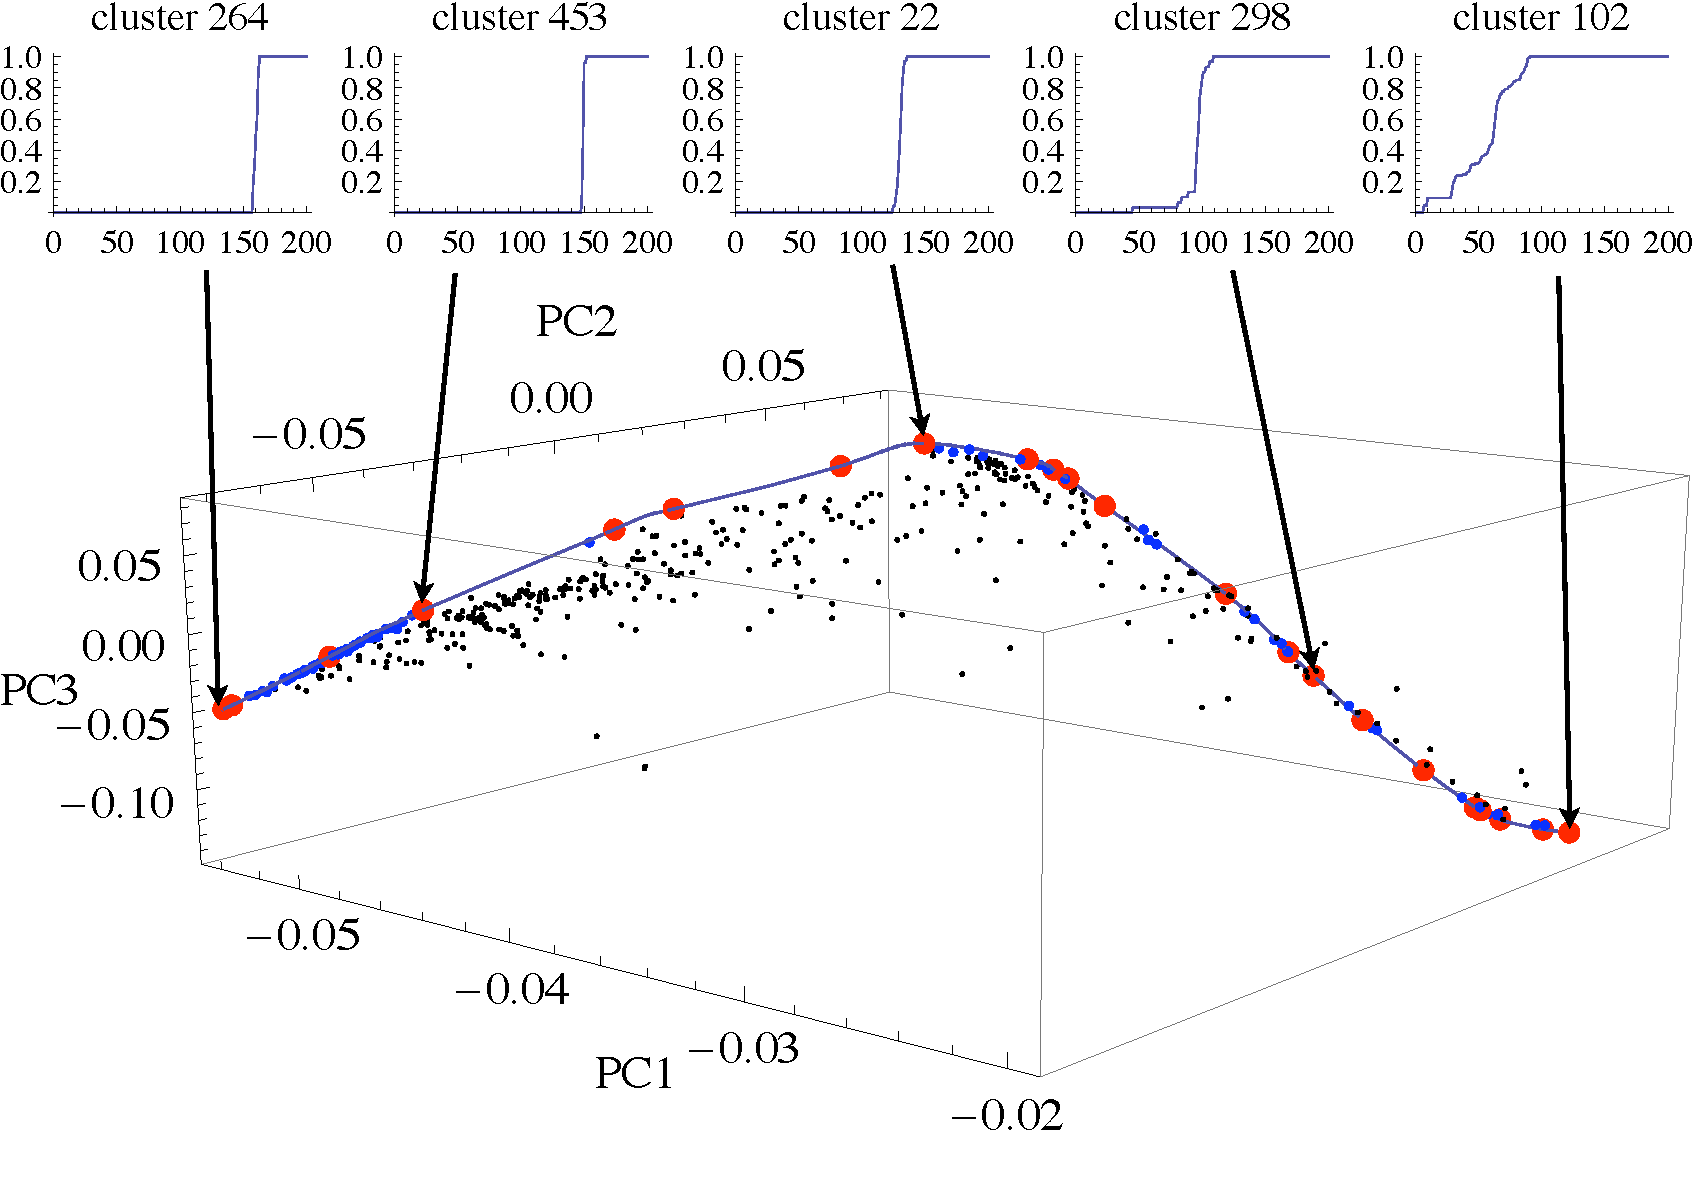
\includegraphics[width=3.5in]{time_pca_3d}%
\caption{Time flowlet clusters projected onto their three most significant principal components ({\footnotesize{PC1}}, {\footnotesize{PC2}}, {\footnotesize{PC3}}). {\footnotesize{CDF}}s of example clusters along the primary ``backbone'' of behaviors are shown above. Backbone clusters are shown as large points and those close to the backbone as medium points. The small points are clusters whose behavior is a weighted combination of those along the backbone.}
\label{fig:time-pca-3d}
\end{center}
\vspace{-2em}
\end{figure}

\section{Conclusions}\label{sec:conclusions}

\section{Acknowledgments}
This work was funded in part by NSF Career Award CNS-0347886 and by NSF NeTS Award CNS-0435527. Special thanks to Matthew Allen, Khaled Harras, Allan Knight, and Rich Wolski for their invaluable help and advice.

\bibliography{IEEE,references}

\end{document}
